\documentclass[aspectratio=169]{beamer}

% LARA: high-level presentation of the ICPM 2027 paper.

\usetheme{Madrid}
\usecolortheme{seahorse}
\usepackage{tikz}
\usetikzlibrary{positioning,fit,backgrounds,arrows.meta,calc}
\usepackage{booktabs}
\usepackage{pgfplots}
\pgfplotsset{compat=1.16}

\definecolor{larablue}{HTML}{2A78D6}
\definecolor{laraaqua}{HTML}{1BAF7A}
\definecolor{laraamber}{HTML}{D97E22}

\setbeamercolor{structure}{fg=larablue}
\setbeamercolor{frametitle}{bg=larablue!12, fg=larablue!50!black}
\setbeamertemplate{navigation symbols}{}
\setbeamertemplate{itemize items}[circle]

\newcommand{\keyc}[1]{\textbf{\textcolor{larablue}{#1}}}
\newcommand{\keyg}[1]{\textbf{\textcolor{laraaqua!70!black}{#1}}}
\newcommand{\keya}[1]{\textbf{\textcolor{laraamber!85!black}{#1}}}

\tikzset{
  iob/.style={draw=black!55, fill=black!4, rounded corners=2.5pt, align=center,
    inner sep=4pt, minimum height=9mm, font=\small},
  lrn/.style={draw=larablue!75!black, fill=larablue!10, rounded corners=2.5pt,
    align=center, inner sep=4pt, minimum height=9mm, font=\small},
  exa/.style={draw=laraaqua!70!black, fill=laraaqua!12, rounded corners=2.5pt,
    align=center, inner sep=4pt, minimum height=9mm, font=\small},
  flow/.style={-{Stealth[length=2.2mm]}, line width=0.9pt, draw=black!60},
  flab/.style={font=\scriptsize, text=black!60, align=center},
  stbg/.style={rounded corners=5pt, inner sep=2.5mm},
  stlab/.style={font=\scriptsize\itshape, inner sep=1.5pt},
}

\title[LARA]{\textbf{LARA}: Learned Alignment with Replay Assurance}
\subtitle{A Reusable Learned Candidate Generator with Exact Certification}
\author[Berti, van der Aalst]{Alessandro Berti \and Wil M.P. van der Aalst}
\institute[PADS, RWTH]{Process and Data Science (PADS), RWTH Aachen University}
\date{ICPM 2027}

\begin{document}

% ---------------------------------------------------------------- 1
\begin{frame}
  \titlepage
\end{frame}

% ---------------------------------------------------------------- 2
\begin{frame}{The Problem}
  \begin{itemize}\setlength{\itemsep}{9pt}
    \item \keyc{Alignments} explain, event by event, how a trace deviates
      from a process model
    \item Optimal alignments need \keya{exact shortest-path search} (A*):
      often the \keya{bottleneck} on real discovered models
    \item Purely \keyc{learned} aligners are fast, but may be
      \keya{illegal} or \keya{silently suboptimal}
  \end{itemize}
  \vspace{5mm}
  \begin{block}{The tension}
    \centering \keyg{trust} (exact, slow) \quad vs.\ \quad \keyc{tractability} (learned, fast)
  \end{block}
\end{frame}

% ---------------------------------------------------------------- 3
\begin{frame}{The Goal}
  \begin{block}{Reusable candidates that stay semantically trustworthy}
    A small neural \keyc{candidate generator}, trained \keyc{once} on synthetic data,
    scores alignment moves for \keyg{any Petri net and any log};
    replay and exact methods \keyg{verify, certify, or repair} every answer.
  \end{block}
  \vspace{4mm}
  \begin{itemize}\setlength{\itemsep}{7pt}
    \item One invariant: \keya{neural output is never a certificate}
    \item Every answer is a \keyg{legal alignment with a known cost};
      optionally a \keyg{certified optimal} one
    \item \keyc{Vocabulary-independent}: no retraining, no configuration per log
  \end{itemize}
\end{frame}

% ---------------------------------------------------------------- 4
\begin{frame}{The Approach at a Glance}
  \begin{center}
  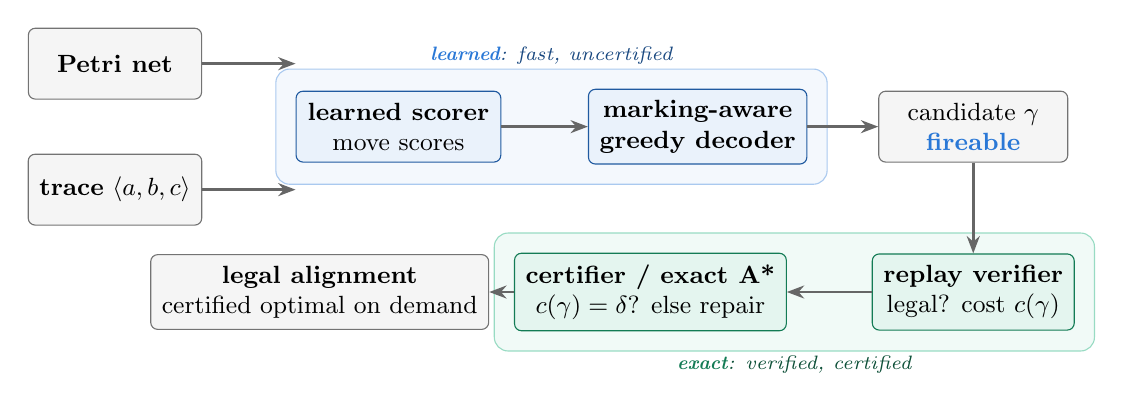
\begin{tikzpicture}[font=\small]
    % inputs
    \node[iob, minimum width=22mm] (net) at (0,0.8) {\textbf{Petri net}};
    \node[iob, minimum width=22mm] (trc) at (0,-0.8) {\textbf{trace} $\langle a,b,c\rangle$};
    % learned stage
    \node[lrn, minimum width=26mm] (fm) at (3.6,0) {\textbf{learned scorer}\\move scores};
    \node[lrn, minimum width=26mm] (dec) at (7.4,0) {\textbf{marking-aware}\\\textbf{greedy decoder}};
    \node[iob, minimum width=24mm] (cand) at (10.9,0) {candidate $\gamma$\\\keyc{fireable}};
    % exact stage
    \node[exa, minimum width=22mm] (ver) at (10.9,-2.1) {\textbf{replay verifier}\\legal? cost $c(\gamma)$};
    \node[exa, minimum width=26mm] (cert) at (6.8,-2.1) {\textbf{certifier / exact A*}\\$c(\gamma) = \delta$? else repair};
    \node[iob, minimum width=26mm] (out) at (2.6,-2.1) {\textbf{legal alignment}\\certified optimal on demand};
    \draw[flow] (net.east) -- (fm.west |- net.east);
    \draw[flow] (trc.east) -- (fm.west |- trc.east);
    \draw[flow] (fm) -- (dec);
    \draw[flow] (dec) -- (cand);
    \draw[flow] (cand) -- (ver);
    \draw[flow] (ver) -- (cert);
    \draw[flow] (cert) -- (out);
    % backgrounds
    \begin{scope}[on background layer]
      \node[stbg, fill=larablue!5, draw=larablue!40, fit=(fm)(dec)] (lbg) {};
      \node[stbg, fill=laraaqua!6, draw=laraaqua!45, fit=(ver)(cert)] (ebg) {};
    \end{scope}
    \node[stlab, text=larablue!60!black, anchor=south] at (lbg.north)
      {\keyc{learned}: fast, uncertified};
    \node[stlab, text=laraaqua!45!black, anchor=north] at (ebg.south)
      {\keyg{exact}: verified, certified};
  \end{tikzpicture}
  \end{center}
  \vspace{2mm}
  \centering
  Degrades from \keyg{certified optimal} to a \keyc{safe upper bound}, \keya{never to wrong}.
\end{frame}

% ---------------------------------------------------------------- 5
\begin{frame}{Architecture of the Learned Scorer}
  \begin{center}
  \resizebox{0.98\textwidth}{!}{%
  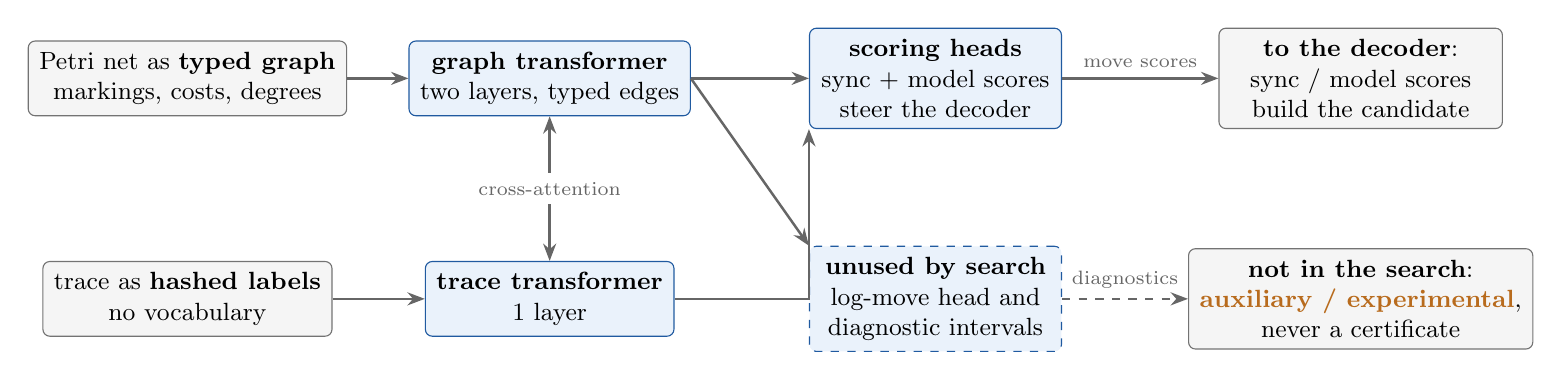
\begin{tikzpicture}[font=\small]
    % inputs
    \node[iob, minimum width=28mm] (g) at (0,1.4) {Petri net as \textbf{typed graph}\\markings, costs, degrees};
    \node[iob, minimum width=28mm] (h) at (0,-1.4) {trace as \textbf{hashed labels}\\no vocabulary};
    % encoders
    \node[lrn, minimum width=30mm] (gt) at (4.6,1.4) {\textbf{graph transformer}\\two layers, typed edges};
    \node[lrn, minimum width=30mm] (tt) at (4.6,-1.4) {\textbf{trace transformer}\\1 layer};
    \draw[flow, {Stealth[length=2.2mm]}-{Stealth[length=2.2mm]}]
      (gt) -- node[flab, fill=white] {cross-attention} (tt);
    % heads
    \node[lrn, minimum width=32mm] (heads) at (9.5,1.4)
      {\textbf{scoring heads}\\sync + model scores\\steer the decoder};
    \node[lrn, minimum width=32mm, dashed] (diag) at (9.5,-1.4)
      {\textbf{unused by search}\\log-move head and\\diagnostic intervals};
    \draw[flow] (g) -- (gt);
    \draw[flow] (h) -- (tt);
    \draw[flow] (gt) -- (heads);
    \draw[flow] (tt) -- (heads.west |- tt) -- (heads.south west);
    \draw[flow] (gt.east) -- (diag.north west);
    % out
    \node[iob, minimum width=36mm] (dec) at (14.9,1.4)
      {\textbf{to the decoder}:\\sync / model scores\\build the candidate};
    \node[iob, minimum width=36mm] (ana) at (14.9,-1.4)
      {\textbf{not in the search}:\\\keya{auxiliary / experimental},\\never a certificate};
    \draw[flow] (heads) -- node[flab, above] {move scores} (dec);
    \draw[flow, dashed] (diag) -- node[flab, above] {diagnostics} (ana);
  \end{tikzpicture}}
  \end{center}
  \vspace{1mm}
  \begin{itemize}\setlength{\itemsep}{4pt}
    \item Coupled encoders: \keyc{two graph layers} plus a \keyc{1-layer}
      trace transformer exchange messages; scores are \keyc{trace-dependent}
    \item The decoder consumes only \keyc{synchronous and model-move} scores;
      the \keya{log-move head} and \keya{diagnostic intervals} do not steer search
    \item Small model: about \keyc{1.7M} parameters, \keyc{two graph layers}
      ($d=96$), runs on \keyc{CPU}
  \end{itemize}
\end{frame}

% ---------------------------------------------------------------- 6
\begin{frame}{Training Loss: Imitating the Exact Aligner}
  The model learns to \keyc{imitate} optimal alignments computed by exact A*:
  \begin{equation*}
    \mathcal{L} \;=\; \underbrace{w_m\,(\mathcal{L}_{\mathrm{sync}}
      + \mathcal{L}_{\mathrm{log}} + \mathcal{L}_{\mathrm{model}})}_{
      \textcolor{larablue}{\textbf{imitation of moves}},\; w_m = 1.0}
    \;+\; \underbrace{w_c\,\mathcal{L}_{\mathrm{cost}}
      + w_b\,\mathcal{L}_{\mathrm{bound}} + w_\ell\,\mathcal{L}_{\mathrm{bal}}
      + w_e\,\mathcal{L}_{\mathrm{ent}}}_{
      \textcolor{laraamber!85!black}{\textbf{unused by search}},\;
      w \le 0.03}
  \end{equation*}
  \vspace{1mm}
  \begin{itemize}\setlength{\itemsep}{5pt}
    \item $\mathcal{L}_{\mathrm{sync}}$: cross-entropy over transition
      \keyc{identities}, not labels: which concrete transition did the optimum
      fire? This is what teaches \keya{duplicate-label} resolution
    \item $\mathcal{L}_{\mathrm{log}}$ / $\mathcal{L}_{\mathrm{model}}$:
      which events did the optimum \keyc{skip}, which transitions did it fire
      \keyc{without a matching event}? Only model scores enter the decoder;
      $\mathcal{L}_{\mathrm{log}}$ is \keya{auxiliary}
    \item $\mathcal{L}_{\mathrm{cost}}$, $\mathcal{L}_{\mathrm{bound}}$,
      $\mathcal{L}_{\mathrm{bal}}$, $\mathcal{L}_{\mathrm{ent}}$ supervise
      experimental intervals and router regularization; they
      \keya{never enter decoding, replay, or exact search}
  \end{itemize}
  \vspace{1mm}
  \centering \small
  Move imitation is dominant; diagnostics and the unused log-move head
  \keya{do not} steer the candidate.
\end{frame}

% ---------------------------------------------------------------- 7
\begin{frame}{From Petri Net + Trace to Transition Likelihoods}
  \begin{center}
  \resizebox{0.98\textwidth}{!}{%
  \begin{tikzpicture}[font=\scriptsize, x=1cm, y=1cm]
    % Petri-net branch
    \node[iob, minimum width=28mm] (net) at (0,1.55)
      {\textbf{typed Petri graph}\\places: $m_0,m_f$, degrees\\transitions: label, $\tau$, costs};
    \node[lrn, minimum width=27mm] (graph) at (3.7,1.55)
      {\textbf{graph transformer}\\two layers; typed arcs\\forward + reverse};
    \node[lrn, minimum width=20mm] (trans) at (7.05,1.55)
      {$h_j\in\mathbb{R}^{96}$\\per transition $t_j$};
    % Trace branch
    \node[iob, minimum width=28mm] (trace) at (0,-1.05)
      {\textbf{trace} $\sigma=\langle a_1,\ldots,a_n\rangle$\\BLAKE2b label ids\\shared with transitions};
    \node[lrn, minimum width=27mm] (seq) at (3.7,-1.05)
      {\textbf{trace transformer}\\1 layer; positions\\global trace context};
    \node[lrn, minimum width=20mm] (events) at (7.05,-1.05)
      {$e_i\in\mathbb{R}^{96}$\\per event $a_i$};
    % Coupling and output
    \draw[flow] (net) -- (graph);
    \draw[flow] (graph) -- (trans);
    \draw[flow] (trace) -- (seq);
    \draw[flow] (seq) -- (events);
    \draw[flow, {Stealth[length=2.2mm]}-{Stealth[length=2.2mm]}]
      (trans) -- node[flab, fill=white, align=center]
      {bidirectional\\cross-attention} (events);
    \node[lrn, minimum width=31mm, minimum height=21mm] (score) at (10.7,0.25)
      {\textbf{label-masked}\\\textbf{bilinear score}\\[1mm]
       $s_{ij}=\dfrac{(W e_i)^\top h_j}{\sqrt{96}}$\\
       $s_{ij}=-\infty$ if $\ell(a_i)\ne\ell(t_j)$};
    \node[exa, minimum width=28mm] (prob) at (14.45,0.25)
      {\textbf{transition likelihood}\\
       $p(t_j\mid a_i,N,\sigma)$\\$=\operatorname{softmax}_j(s_{ij})$};
    \draw[flow] (trans.east) -- (score.north west);
    \draw[flow] (events.east) -- (score.south west);
    \draw[flow] (score) -- (prob);
  \end{tikzpicture}}
  \end{center}
  \vspace{0.5mm}
  \small
  \begin{itemize}\setlength{\itemsep}{2pt}
    \item The net encoder makes each $h_j$ identify a \keyc{concrete transition}
      by initial/final markings, routing, and downstream context---not merely
      by its label.
    \item Cross-attention makes both $h_j$ and $e_i$ depend on the \keyc{whole
      net--trace pair}; the same transition can therefore score differently for
      different trace suffixes.
    \item The hard mask gives mismatched labels probability zero; among
      duplicates, the softmax ranks \keyc{transition identities}. During decoding,
      the current marking further restricts the choice to \keyg{enabled transitions}.
  \end{itemize}
\end{frame}

% ---------------------------------------------------------------- 8
\begin{frame}{Where Learning Helps: Duplicate Labels}
  \begin{columns}[T]
  \begin{column}{0.54\textwidth}
    \small
    The decoder reads the trace \keyc{one event at a time}, always knowing
    the \keyc{current marking} of the Petri net:
    \begin{itemize}\setlength{\itemsep}{4pt}
      \item If exactly \keyg{one} enabled transition carries the event's label,
        the choice is \keyg{forced by the Petri net}: no learning needed
      \item If \keyc{several} enabled transitions carry the same label,
        the learned \keyc{synchronous score} decides which concrete
        transition the event refers to
      \item If \keyc{no} such transition is enabled, the \keyc{model-move
        scores} guide a short search that lets the Petri net catch up
      \item If even that fails, the event is a deviation:
        it becomes a \keya{log move} (the log-move head is unused)
    \end{itemize}
  \end{column}
  \begin{column}{0.42\textwidth}
    \begin{center}
    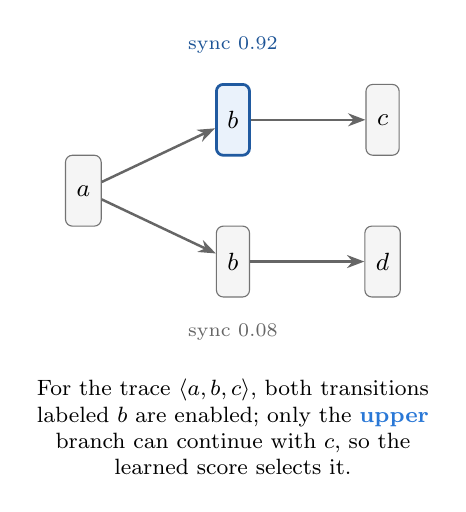
\begin{tikzpicture}[font=\small]
      \node[iob] (p1) at (0,0) {$a$};
      \node[lrn, draw=larablue!75!black, line width=1pt] (b1) at (1.9,0.9) {$b$};
      \node[iob] (b2) at (1.9,-0.9) {$b$};
      \node[iob] (c) at (3.8,0.9) {$c$};
      \node[iob] (d) at (3.8,-0.9) {$d$};
      \draw[flow] (p1) -- (b1); \draw[flow] (p1) -- (b2);
      \draw[flow] (b1) -- (c); \draw[flow] (b2) -- (d);
      \node[flab, text=larablue!70!black] at (1.9,1.85) {sync $0.92$};
      \node[flab] at (1.9,-1.8) {sync $0.08$};
      \node[font=\footnotesize, align=center] at (1.9,-3.0)
        {For the trace $\langle a, b, c\rangle$, both transitions\\
         labeled $b$ are enabled; only the \keyc{upper}\\
         branch can continue with $c$, so the\\
         learned score selects it.};
    \end{tikzpicture}
    \end{center}
  \end{column}
  \end{columns}
  \vspace{1mm}
  \centering \small
  The candidate is always \keyg{replayable}; \keyg{optimality} is checked by the exact layer.
\end{frame}

% ---------------------------------------------------------------- 9
\begin{frame}{Training and Validation Data}
  \textbf{Exact-labeled behavior families} (imitation of the exact aligner):
  \vspace{2mm}
  \begin{enumerate}\setlength{\itemsep}{5pt}
    \item \keyc{draw a family}: one visible behavior, two Petri-net encodings,
      two shared traces (four rows); four equally weighted motifs
      (ordinary tree, duplicate/silent, concurrency, M pattern)
    \item \keyc{perturb} most traces with 1--3 deletions, insertions,
      substitutions, repetitions, swaps, or truncations (20\% stay clean)
    \item \keyc{label} with exact A*: optimal alignment \keyg{with transition identities},
      replay-verified
  \end{enumerate}
  \vspace{3mm}
  \begin{columns}[T]
  \begin{column}{0.5\textwidth}
    \begin{center}
    \begin{tabular}{lr}
      \toprule
      Split & Examples \\
      \midrule
      \keyc{Training} & 2,048 \\
      \keyc{Validation} & 512 \\
      \keyc{Test} & 512 \\
      \bottomrule
    \end{tabular}
    \end{center}
  \end{column}
  \begin{column}{0.46\textwidth}
    \small
    \keyc{Hashed labels} $\Rightarrow$ the model learns \keyg{structure},
    never vocabulary: one checkpoint for any log.\\[2mm]
    Corpus \keyc{2,048 / 512 / 512}. Best validation loss at
    \keyc{epoch 49 of 50}, about 41\,s each, \keyc{single CPU}.
  \end{column}
\end{columns}
\end{frame}

% ---------------------------------------------------------------- 10
\begin{frame}{Evaluation: How}
  \small
  \textbf{Protocol}: all runs on a \keyc{single CPU}. LARA always in
  \keyc{fast mode}: the verified neural candidate is scored \keya{as is},
  never repaired, so no exact result contaminates the learned metrics.
  The \keyg{exact A* optimum} $\delta$ is the ground truth for every sample.
  \vspace{2mm}
  \begin{itemize}\setlength{\itemsep}{6pt}
    \item \keyc{In-distribution quality}: 512 held-out rows from unseen
      behavior families; measures whether every candidate is
      \keyg{legal} (replayable), how often its cost \keyg{equals} the
      optimum $\delta$, and \keyg{how far off} it is otherwise
    \item \keyc{Guidance ablation}: identical inputs, but the neural scores are
      replaced by fixed structural tie-breaks; isolates what \keyg{learning}
      adds over constrained search alone
    \item \keyc{Scaling and approximations}: random block-structured Petri nets
      never seen in training, plus PM4Py approximations on the same grids
    \item \keyc{Zero-shot real life}: two public logs (building permits,
      road traffic fines) with Petri nets discovered by the inductive miner;
      \keya{unseen vocabularies, no fine-tuning}
  \end{itemize}
\end{frame}

% ---------------------------------------------------------------- 11
\begin{frame}{Evaluation: Results}
  \begin{columns}[T]
  \begin{column}{0.5\textwidth}
    \begin{center}
    \small
    \begin{tabular}{lr}
      \toprule
      In-distribution ($n = 512$) & \\
      \midrule
      legal alignments & \keyg{100\%} \\
      already optimal & \keyc{91.0\%} \\
      mean cost gap & 0.18 \\
      \bottomrule
    \end{tabular}
    \end{center}
    \vspace{2mm}
    \small Ablation: learning adds \keyc{$+$4.1} overall and
    \keyc{$+$26.6} on \keya{duplicate-prefix} nets
    (95.3\% vs.\ 68.8\%); it also keeps quality
    \keyg{identifier-stable} at 84.4\%.
  \end{column}
  \begin{column}{0.46\textwidth}
    \begin{itemize}\setlength{\itemsep}{5pt}
      \item \keyg{Legality transfers everywhere}: 100\% on unseen families
        and real logs
      \item Fast path stays at \keyc{4.6--8.7\,ms}; at size 40,
        \keya{30--44\%} optimal, but faster than exact A*
      \item Receipt (invisible-heavy): \keyc{16.0 vs.\ 31.0\,ms}
        and \keyc{6.7 vs.\ 12.7\,ms}
      \item Established Petri-net approximations
        \keya{generally return better candidates}
    \end{itemize}
  \end{column}
  \end{columns}
\end{frame}

% ---------------------------------------------------------------- 12
\begin{frame}{Why Consider LARA in Process Mining?}
  \begin{block}{A reusable candidate plus replay and exact certification,
    not a replacement for exact or classical aligners.}
    \centering
    \keyc{learned proposal} $\longrightarrow$ \keyg{replay check}
    $\longrightarrow$ \keyg{exact certificate or repair}
  \end{block}
  \vspace{2mm}
  \begin{columns}[T]
  \begin{column}{0.31\textwidth}
    \centering \keyc{Portable first result}\par
    \vspace{1mm}\small
    One vocabulary-independent checkpoint proposes a legal candidate
    with predictable latency; the fast path overtakes A* on harder
    tested models and the receipt nets.
  \end{column}
  \begin{column}{0.31\textwidth}
    \centering \keyg{Same conformance object}\par
    \vspace{1mm}\small
    The output is still an event-by-event, transition-identity alignment with
    a replay-verified cost---usable by existing diagnostics, not an opaque
    fitness prediction.
  \end{column}
  \begin{column}{0.31\textwidth}
    \centering \keya{Narrower learning gain}\par
    \vspace{1mm}\small
    Learning pays on \keyc{duplicate prefixes} and
    \keyc{identifier-stable scoring}. Marking-aware search is already
    strong; classical approximations usually have better quality.
  \end{column}
  \end{columns}
  \vspace{4mm}
  \centering
  \textbf{Practical role:} a reusable proposal in front of replay and the
  exact aligner, \keya{not a replacement for formal guarantees}.
\end{frame}

% ---------------------------------------------------------------- 13
\begin{frame}{What Can Be Improved}
  \begin{itemize}\setlength{\itemsep}{8pt}
    \item Quality does \keya{not transfer to large Petri nets}
      (30--44\% optimal at size 40): classical approximations stay
      much closer to the optimum; broader training and stronger
      decoding are the next steps
    \item The decoder never compares the trained \keya{log-move score}
      with catch-up paths, and it never revises an early commitment:
      joint ranking and beam search are the direct improvements
    \item Only \keya{two real-life logs} tested, and certified mode
      still runs exact A* on every trace: no end-to-end certified speedup
      is demonstrated
  \end{itemize}
\end{frame}

% ---------------------------------------------------------------- 14
\begin{frame}{Takeaway}
  \begin{block}{}
    \centering \keyc{Learning proposes}, \keyg{exact reasoning certifies}:
    the result is \keyg{never less trustworthy} than classical alignment.
  \end{block}
  \vspace{2mm}
  \small
  \begin{itemize}\setlength{\itemsep}{6pt}
    \item \keyg{Legality is unconditional}: every produced alignment can be
      replayed from the initial to the final marking, and this held in
      \keyg{100\%} of the cases on synthetic families, on larger unseen
      Petri nets, and on real-life logs alike
    \item \keyc{91.0\%} of the 512-row test split already carry the
      \keyc{exact optimal cost}; the other 9.0\% are \keyg{repaired exactly},
      never returned wrong. Certified mode still invokes A* on every trace
    \item Learning pays on \keya{duplicate prefixes}
      (\keyc{95.3\%} vs.\ 68.8\%, $+26.6$) and keeps ordinary-tree quality
      \keyc{identifier-stable} at 84.4\%; overall $+4.1$.
      Approximations generally beat this candidate quality
    \item The fast path stays at \keyc{4.6--8.7\,ms} and overtakes exact A*
      on larger stress nets; on receipt it is
      \keyc{16.0 vs.\ 31.0\,ms} and \keyc{6.7 vs.\ 12.7\,ms}
  \end{itemize}
  \vspace{1mm}
  \centering\small Checkpoint, scripts, and results:
  \url{https://github.com/fit-alessandro-berti/lara-align}
\end{frame}

% ================================================================ appendix
\appendix

\begin{frame}
  \centering
  {\LARGE \textbf{\textcolor{larablue}{Appendix}}}\\[3mm]
  {\large Detailed Evaluation Results}\\[5mm]
  \small LARA always in fast mode; exact A* optimum as ground truth.
\end{frame}

% ---------------------------------------------------------------- A2
\begin{frame}{Appendix: In-Distribution Results}
  \begin{columns}[T]
  \begin{column}{0.46\textwidth}
    \vspace{2mm}
    \begin{center}
    \small
    \begin{tabular}{lr}
      \toprule
      Held-out test split ($n = 512$) & \\
      \midrule
      replayable (legal) & \keyg{100.0\%} \\
      already optimal / no repair & \keyc{91.0\%} \\
      exact transition-sequence match & 61.1\% \\
      mean / median cost gap & 0.18 / 0.00 \\
      p90 / p95 / max cost gap & 0.0 / 2.0 / 4.0 \\
      \bottomrule
    \end{tabular}
    \end{center}
    \vspace{3mm}
    \small 466 of 512 candidates are optimal; 95\% lie within two
    cost units, and \keya{no gap exceeds four}. Sequence match is
    lower because several legal alignments can share the same cost.
  \end{column}
  \begin{column}{0.5\textwidth}
    \begin{center}
    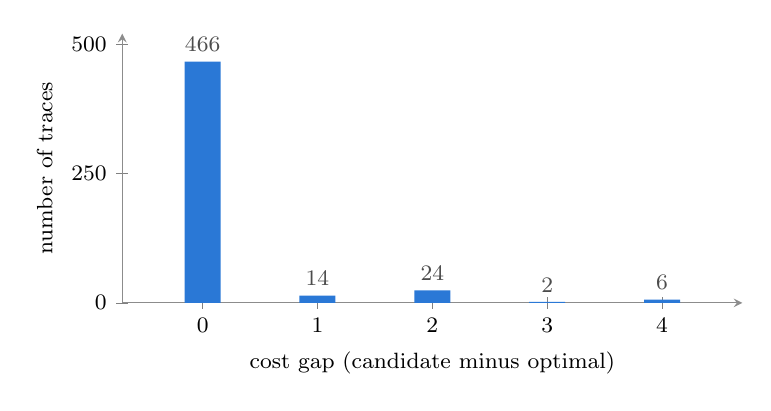
\begin{tikzpicture}
    \begin{axis}[
      ybar, bar width=13pt,
      width=0.78\linewidth, height=5.0cm,
      xlabel={cost gap (candidate minus optimal)},
      ylabel={number of traces},
      xmin=-0.7, xmax=4.7, ymin=0, ymax=520,
      xtick={0,1,2,3,4},
      ytick={0,250,500},
      axis lines=left, axis line style={black!45},
      ticklabel style={font=\footnotesize},
      label style={font=\footnotesize},
      nodes near coords,
      every node near coord/.append style={font=\footnotesize, color=black!70},
    ]
    \addplot[fill=larablue, draw=none] coordinates {(0,466)(1,14)(2,24)(3,2)(4,6)};
    \end{axis}
    \end{tikzpicture}
    \end{center}
  \end{column}
  \end{columns}
\end{frame}

% ---------------------------------------------------------------- A3
\begin{frame}{Appendix: Guidance Ablation}
  Identical inputs and decoder; only the neural scores are replaced by fixed
  structural tie-breaks:
  \vspace{2mm}
  \begin{center}
  \small
  \begin{tabular}{lrrr}
    \toprule
    Metric ($n = 512$) & unguided & guided & $\Delta$ \\
    \midrule
    replayable & 100.0\% & 100.0\% & 0.0 \\
    equal to optimum cost & 86.9\% & \keyc{91.0\%} & $+4.1$ \\
    exact transition-sequence match & 57.8\% & \keyc{61.1\%} & $+3.3$ \\
    mean cost gap & 0.26 & \keyc{0.18} & $-$0.08 \\
    duplicate-prefix, optimal & 68.8\% & \keyc{95.3\%} & \keyg{$+$26.6} \\
    ordinary tree, isomorphic rename & 76.6\% & \keyc{84.4\%} & $+7.8$ \\
    \bottomrule
  \end{tabular}
  \end{center}
  \vspace{2mm}
  \begin{itemize}\setlength{\itemsep}{4pt}
    \item On most motifs, marking-aware search already determines the
      candidate; guidance changes \keya{no cost} for silent routing,
      concurrency, or either M representation
    \item Learning's documented gains are \keyc{duplicate-prefix}
      disambiguation and \keyg{identifier-stable} scoring (84.4\% on
      both the canonical tree and its rename)
  \end{itemize}
\end{frame}

% ---------------------------------------------------------------- A4
\begin{frame}{Appendix: Scaling Benchmark}
  Random block-structured Petri nets, \keya{never seen in training}
  (10 samples per configuration, 30\,s exact timeout):
  \vspace{1mm}
  \begin{columns}[T]
  \begin{column}{0.52\textwidth}
    \begin{center}
    \footnotesize
    \begin{tabular}{rrrrr}
      \toprule
      size / dev. & legal & optimal & fast med. & exact med. \\
      \midrule
       5 / 0.15 & 100\% & 90\% & 5.5 ms & 1.3 ms \\
      10 / 0.15 & 100\% & 80\% & 5.0 ms & 1.8 ms \\
      20 / 0.15 & 100\% & 60\% & 6.9 ms & 2.9 ms \\
      40 / 0.15 & 100\% & 30\% & 8.7 ms & \keya{63.9 ms} \\
      40 / 0.35 & 100\% & 44\% & 8.6 ms & 24.7 ms \\
      \bottomrule
    \end{tabular}
    \end{center}
    \vspace{1.5mm}
    \small Fast path stays at \keyc{4.6--8.7\,ms};
    at size 40, \keya{30--44\%} optimal.
    \keyg{Legality is scale-invariant}.
    Crossover near \keyc{size 40} (dev.\ 0.15); first exact
    \keya{timeout} appears there (dev.\ 0.35).
  \end{column}
  \begin{column}{0.44\textwidth}
    \begin{center}
    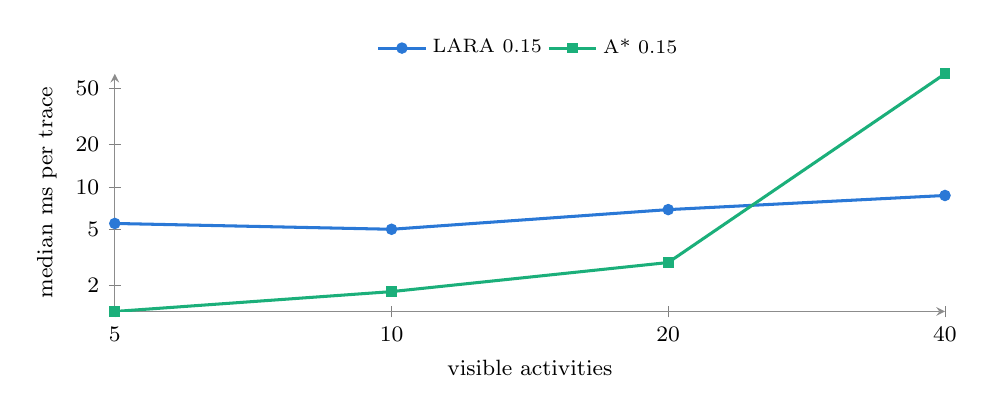
\begin{tikzpicture}
    \begin{axis}[
      width=\linewidth, height=4.6cm,
      xlabel={visible activities},
      ylabel={median ms per trace},
      xmode=log, log ticks with fixed point, xtick={5,10,20,40},
      ymode=log, log ticks with fixed point, ytick={1,2,5,10,20,50},
      axis lines=left, axis line style={black!45},
      ticklabel style={font=\footnotesize},
      label style={font=\footnotesize},
      legend style={draw=none, fill=none, font=\scriptsize,
        at={(0.5,1.02)}, anchor=south, legend columns=2},
      every axis plot/.append style={line width=1.1pt},
    ]
    \addplot[larablue, mark=*, mark size=1.5pt]
      coordinates {(5,5.5)(10,5.0)(20,6.9)(40,8.7)};
    \addlegendentry{LARA 0.15}
    \addplot[laraaqua, mark=square*, mark size=1.4pt]
      coordinates {(5,1.3)(10,1.8)(20,2.9)(40,63.9)};
    \addlegendentry{A* 0.15}
    \end{axis}
    \end{tikzpicture}
    \end{center}
  \end{column}
  \end{columns}
\end{frame}

% ---------------------------------------------------------------- A5
\begin{frame}{Appendix: Zero-Shot Results on Real-Life Logs}
  Same checkpoint, \keya{no fine-tuning}; Petri nets discovered by the
  inductive miner (noise 0.0 $=$ perfectly fitting, 0.5 $=$ filtered):
  \vspace{2mm}
  \begin{center}
  \footnotesize
  \begin{tabular}{llrrrr}
    \toprule
    Log & Noise & Legal & Optimal (trace-wtd.) & Max gap & Median LARA / exact \\
    \midrule
    road traffic & 0.0 & \keyg{100\%} & 100.0\% & 0 & 5.4 / 1.9 ms \\
    road traffic & 0.5 & \keyg{100\%} & 94.0\%  & 3 & 5.2 / 1.6 ms \\
    receipt      & 0.0 & \keyg{100\%} & 82.6\%  & 5 & \keyc{16.0 / 31.0 ms} \\
    receipt      & 0.5 & \keyg{100\%} & 74.6\%  & 7 & \keyc{6.7 / 12.7 ms} \\
    \bottomrule
  \end{tabular}
  \end{center}
  \vspace{3mm}
  \begin{itemize}\setlength{\itemsep}{5pt}
    \item \keyg{Legality transfers perfectly} to unseen vocabularies and
      invisible-heavy discovered models (47 invisible vs.\ 27 visible
      transitions on the fitting receipt net)
    \item Optimality is stronger when weighted by traces; misses concentrate
      in \keya{rare, long variants} and remain safe upper bounds
    \item Guided and unguided quality coincide here: these nets have
      \keya{no duplicate labels}, so the scorer's main ambiguity gain is
      not exercised
  \end{itemize}
\end{frame}

% ---------------------------------------------------------------- A6
\begin{frame}{Appendix: Approximations Beat Current Candidate Quality}
  Independent replay of PM4Py approximations vs.\ LARA on the same
  held-out split and stress grid:
  \vspace{2mm}
  \begin{center}
  \small
  \begin{tabular}{lrrrr}
    \toprule
    Method & Held-out opt. & Held-out gap & Stress opt. & Stress med. \\
    \midrule
    LARA guided & 91.0\% & 0.180 & 59.5\% & 7.69 ms \\
    discounted A* & 95.7\% & 0.090 & 75.9\% & 1.17 ms \\
    tandem repeats & 98.0\% & 0.039 & 93.6\% & 1.37 ms \\
    sliding window & 100.0\% & 0.000 & 100.0\% & 1.27 ms \\
    fixed horizon & 98.0\% & 0.047 & 82.9\% & 82.37 ms \\
    \bottomrule
  \end{tabular}
  \end{center}
  \vspace{3mm}
  \begin{itemize}\setlength{\itemsep}{5pt}
    \item All tested Petri-net approximations beat LARA's exact-cost rate
      on held-out data; sliding window is perfect because every test
      trace fits one window of 20 events
    \item LARA's distinct advantage is \keyc{coverage} (legal in every case)
      plus a \keyg{reusable scorer} behind an explicit trust boundary
    \item The current decoder is \keya{not} claimed to replace exact A*
      or these approximations
  \end{itemize}
\end{frame}

\end{document}
